\documentclass[25pt, portrait]{tikzposter}
\title{\parbox{.85\textwidth}{\centering Time-dependent calculation of intersystem crossing rates of sulfur-substituted adamantane derivatives\vspace{.85cm}}}
\author{Robert Scholz and Peter Saalfrank}
\institute{\Large Theoretische Chemie, Institut f\"ur Chemie, Universit\"at Potsdam, Karl-Liebknecht-Str. 24-25, D-14476 Potsdam}
\usepackage{tikz}
\usepackage{adjustbox}
\usepackage{textcomp}
\usepackage{multicol}
\usetikzlibrary{shapes, arrows.meta}
% \tikzstyle{block} = [rectangle, draw, fill=blue!25, 
%     text width=7cm, text centered, rounded corners, minimum height=2cm]
% \tikzstyle{wideblock} = [rectangle, draw, fill=blue!25, 
%     text width=12cm, text centered, rounded corners, minimum height=2cm]   
% \tikzstyle{line} = [ultra thick, arrows={-stealth[scale=10]}]
\usetheme{Default}

\makeatletter
\renewenvironment{tikzfigure}[1][]{
  \def \rememberparameter{#1}
  \vspace{10pt}
  \refstepcounter{figurecounter}
  \begin{center}
  }{
    \ifx\rememberparameter\@empty
    \else %nothing
    \\[10pt]
    {\large Fig.~\thefigurecounter: \rememberparameter}
    \fi
  \end{center}
}
\makeatother

\begin{document}

\maketitle[width=.9\textwidth]
%   \block{Basic Block}{Text}
  \begin{columns}
    
    \column{0.355}
      \block{Introduction}{
% 	For \textit{in vivo} bioimaging, sulfur derivatives of diamondoids may serve as an alternative to conventional dye molecules and quantum dots.
	\begin{itemize}
	  \item	for \textit{in vivo} bioimaging, sulfur derivatives of diamondoids may serve as alternative \cite{optical_gap_sulfur} to %conventional dye molecules~(toxic, less stable) or quantum dots~(too large, could disturb function of target) \cite{optical_gap_sulfur}.  

	  \begin{itemize}
	    \item conventional dye molecules~(often toxic, less photostable)
	    \item quantum dots~(too large, could disturb function of target)
	  \end{itemize}

% 	  \vspace{7cm}
% 	  \item Conventional dye molecules are often toxic and typically have low photostability, due to extended $\pi$-systems. 
% 	  \item Quantum dots usually have thick passivation layers, resulting in a large size ($\sim$10\,nm), potentially interfering with the normal function of the biomolecules of interest.

	  \end{itemize}
	  \begin{minipage}[t]{0.5\colwidth}
	    \begin{itemize}
	      \item diamondoids:$\;$highly$\;$photostable, non-toxic, small size
	      \item problem: optical gap of pristine diamondoids lies in UV region
	      \begin{itemize}
	      \item replacing CH$_2$ with C=S \\$\Rightarrow$ shift to vis (even IR) \cite{optical_gap_sulfur, bachelor}
	      \item but additional S-atoms \\enhance spin-orbit coupling \\$\Rightarrow$ potentially detrimental for role as flourescence marker
	      \end{itemize}
	    \end{itemize}   
	  \end{minipage}
	  \begin{minipage}[t]{0.0005\colwidth}
	    ~
	  \end{minipage}
	  \begin{adjustbox}{valign=t}
	    \begin{minipage}[t]{0.441\colwidth}
	      \begin{tikzfigure}[Optical gap decrease with no. of C=S groups \cite{optical_gap_sulfur}.]
		\includegraphics[width=.41\colwidth]{abb/optical_gap_modified.png}
	      \end{tikzfigure}
	    \end{minipage}
	  \end{adjustbox}
% 	  \item 	Adamantane is the smallest representative of the class of diamondoids
      }
%       \note[targetoffsety=5.5cm, connection, angle=-155, radius=10cm,  width=14cm, innersep=.4cm, rotate=-1.5]{Conventional dye molecules are often toxic and typically have low photostability, due to extended $\pi$-systems.}
%       \note[targetoffsetx=10cm, targetoffsety=5.5cm, connection, angle=-100, radius=5cm,  width=18cm, innersep=.4cm, rotate=1.5]{Because of thick passivation layers, quantum dots usually have a large size ($\sim$10\,nm),  \\hence they may disturb the normal function of marked biomolecules}
	\block{Investigated systems}{
% 	  \begin{minipage}{\colwidth} %frame minipage for 2 minipages
% 
% 	    \begin{minipage}[t]{0.2\colwidth}

% 	    \end{minipage}
		\begin{itemize}
		  \item six thione derivatives of adamantane (smallest diamondoid):
		\end{itemize}

 	  	    
	      \begin{minipage}[t]{0.53 \colwidth}  


	      \begin{tikzfigure}[Adamantane thione and the two di- and three trithiones.]
		\begin{tikzpicture}[node distance= .12\colwidth]
		  \node (adathio) {\includegraphics[width=.24\colwidth]{abb/ada_thio.png}};
		  \node [right of=adathio, yshift=.06\colwidth, xshift=.09\colwidth] (di24) {\includegraphics[width=.12\colwidth]{abb/24dithio.png}};
		  \node [right of=di24] (di26) {\includegraphics[width=.12\colwidth]{abb/26dithio.png}};
		  \node [below of=di24, xshift=-.06\colwidth] (tria6) {\includegraphics[width=.12\colwidth]{abb/246trithio.png}};		  
		  \node [right of=tria6] (trib9) {\includegraphics[width=.12\colwidth]{abb/249trithio.png}};
		  \node [right of=trib9] (tric10) {\includegraphics[width=.12\colwidth]{abb/2410trithio.png}};
		\end{tikzpicture}
	      \end{tikzfigure} 	  
 	  
		  
	    \begin{itemize}  
	      \item focus on intersystem crossing\\ between S$_1\,/\,$T$_1$ and T$_1\,/\,$S$_0$
	      \item adamantane thione also S$_2${}$\,\rightarrow\,${}T$_1$ %(S$_1\,$=$\,$dark) 
	    \end{itemize}   
	  \end{minipage}
	  \begin{adjustbox}{valign=t}
	    \begin{minipage}[t]{0.42\colwidth}
	      \begin{tikzfigure}[Experimental excitation energies of adamantane thione \cite{falk1990}.]
		\includegraphics[width=.255\colwidth]{abb/ada_energy_exp.png}
	      \end{tikzfigure}
	    \end{minipage}
	  \end{adjustbox}
	 \coloredbox{
	              Note, T$_1$ here always means $^3$(n$\,\rightarrow\,${}$\pi^*$), but in exp.$\;$it is T$_2$, \\as $^3$($\pi${}$\,\rightarrow\,${}$\pi^*$) is $\approx500\,$cm$^{-1}$ lower, even in unpolar media  \cite{falk1990}.
	             
		}
	}
      
      \block{Methodology}{
		  \begin{center}
      	\coloredbox[width=.46\colwidth]{work flow for each transition:}
\vspace{0.5cm}
% 		  \begin{center}
%       	\begin{tikzfigure}
	  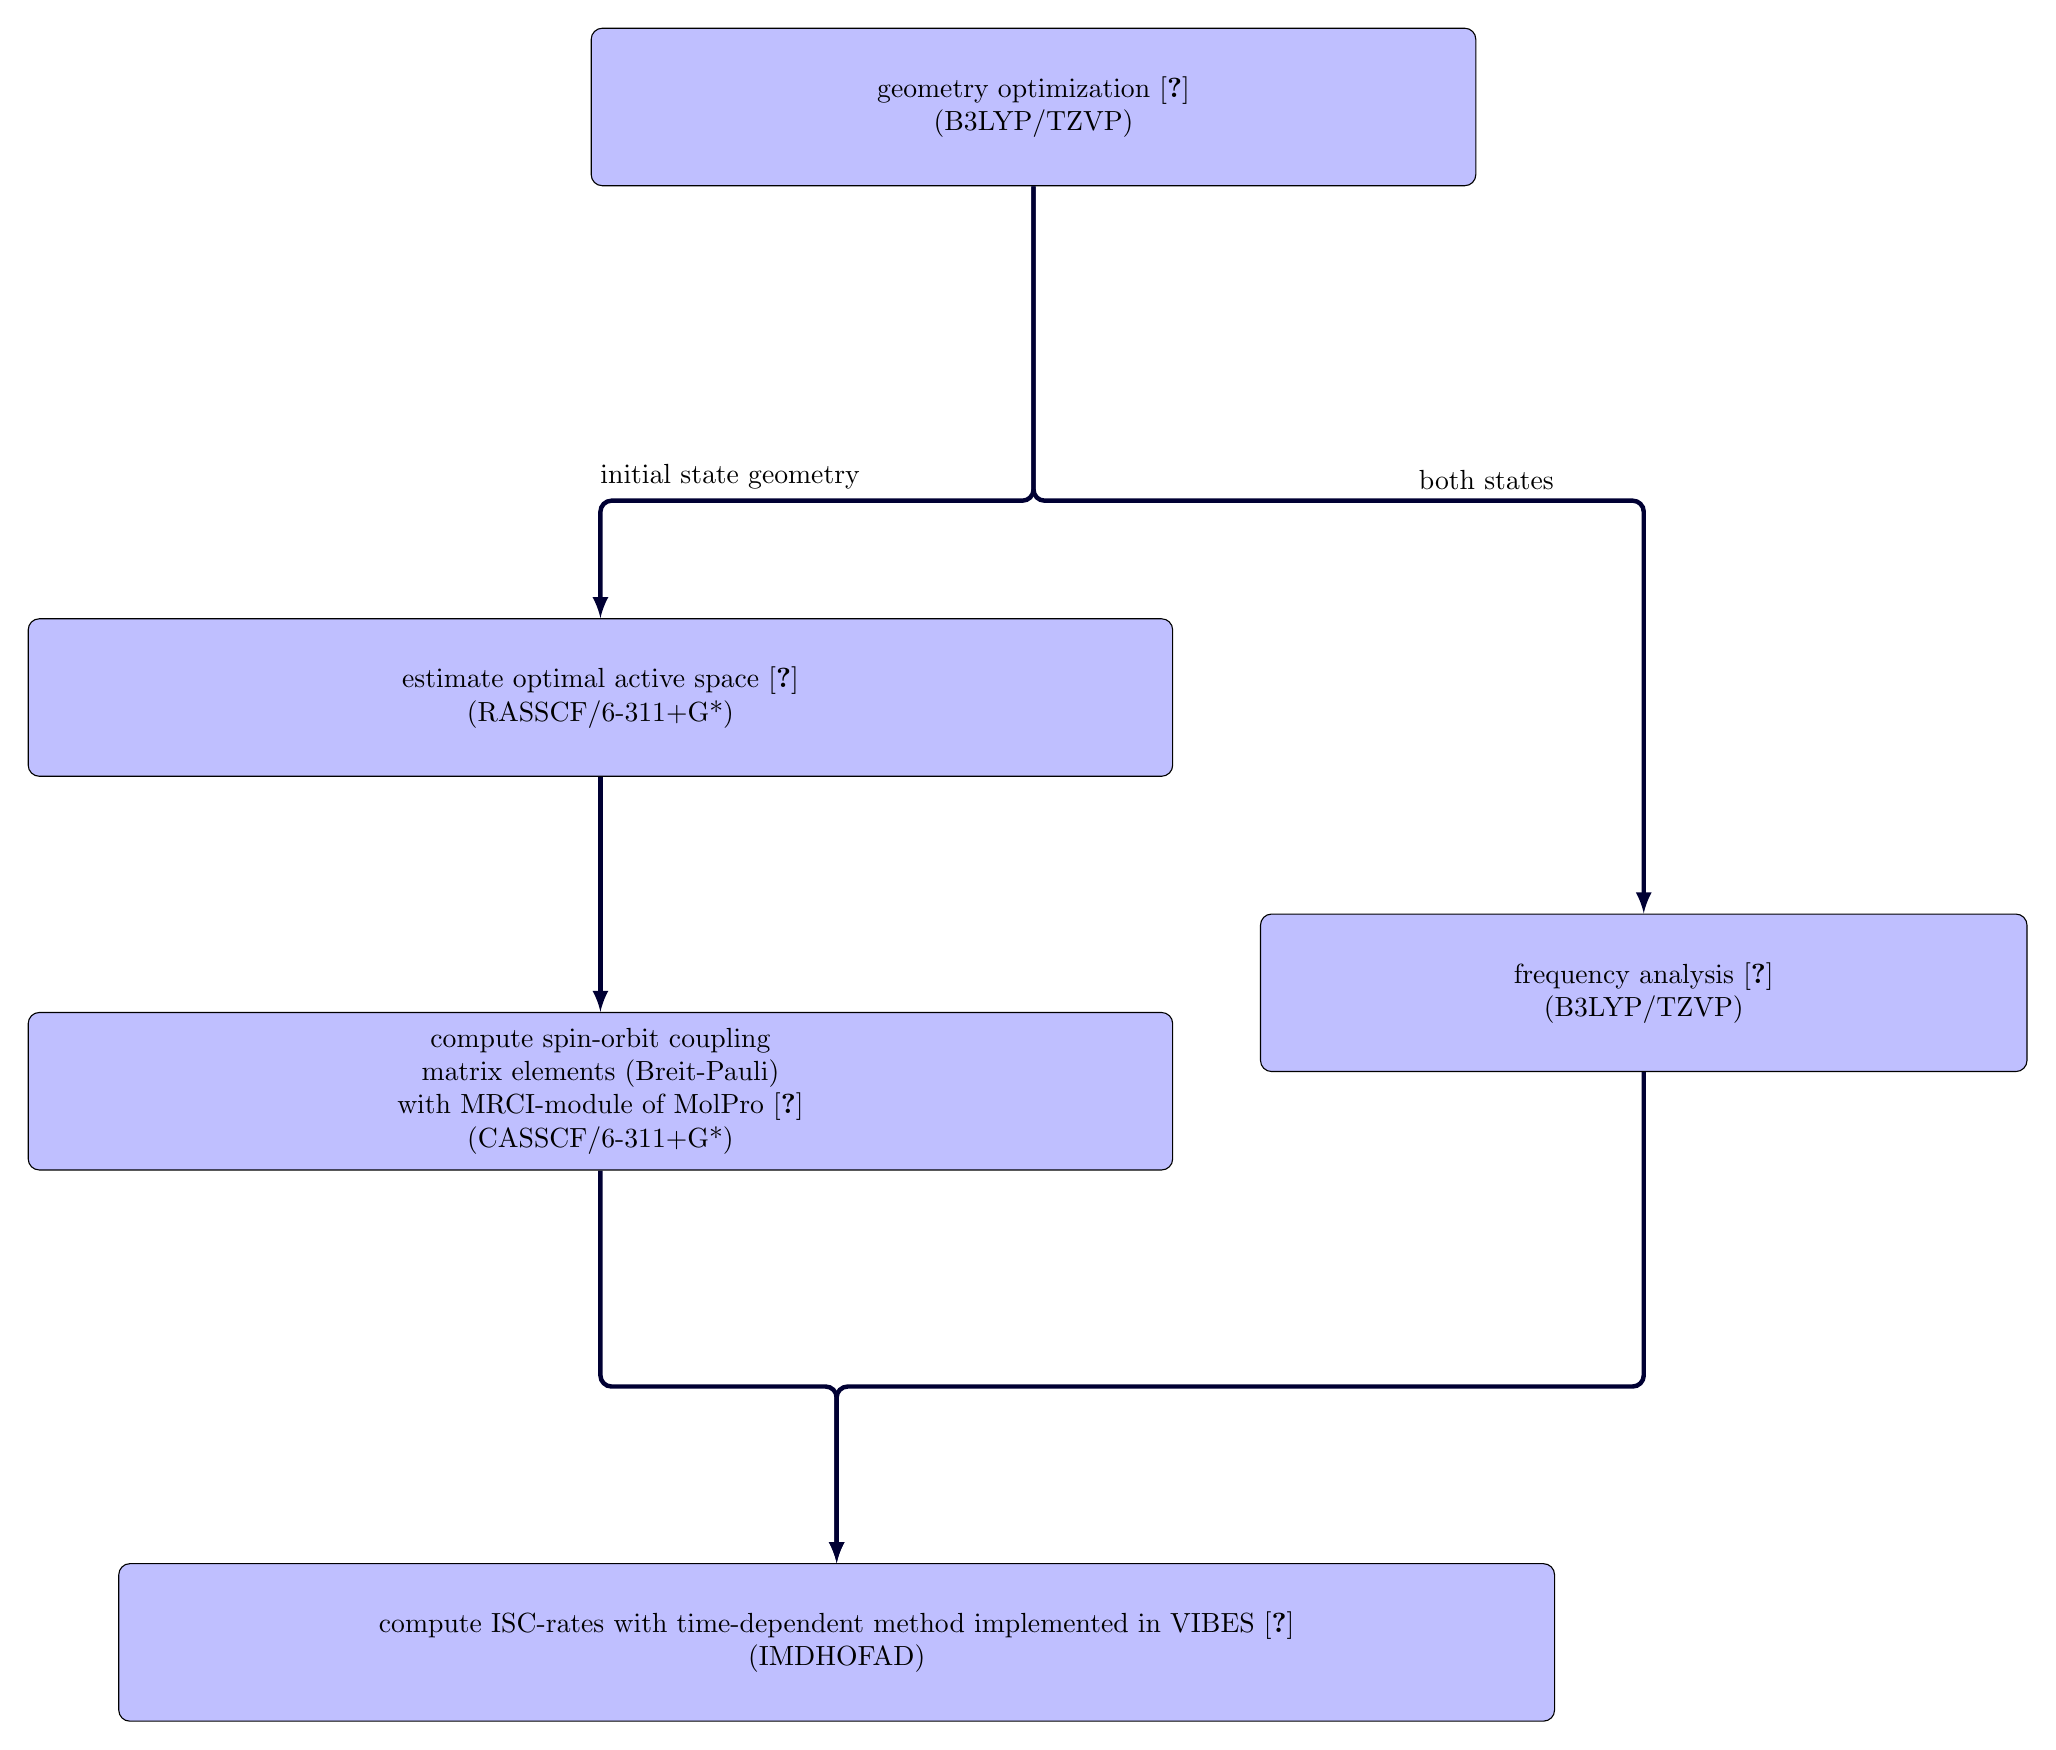
\begin{tikzpicture}
	  [node distance = 9cm,  auto, 
	  %
% 	  wideblock/.style={rectangle, draw, fill=blue!25, text width=12cm, text centered, rounded corners, minimum height=2cm}, 
	  %
	  block/.style={rectangle, draw, fill=blue!25, text width=8cm, text centered, rounded corners, minimum height=2cm}, 
	  %
	  customline/.style={draw = blue!20!black, rounded corners,  ultra thick, arrows={-latex[length=20pt]}}, 
	  %
	  customrev/.style={draw = blue!20!black, rounded corners,  ultra thick, arrows={latex[length=20pt]-}}]
	  
	    \node [block, text width=11cm] (geoopt) {geometry optimization \cite{gauss}\\ (B3LYP/TZVP)};
% 		 \node [below of=geoopt, yshift=5cm] (connector1) {};
	    \node [block, below of=geoopt, yshift=-2.25cm, xshift=7.75cm, text width=9.5cm] (freq) {frequency analysis \cite{gauss} \\(B3LYP/TZVP)};
	    \node [block, below of=geoopt, xshift=-5.5cm, yshift=1.5cm, text width=14.3cm] (ras) {estimate  optimal active space \cite{molpro}\\(RASSCF/6-311+G*)};
	    \node [block, below of=ras, yshift=4cm, text width=14.3cm] (cas) {compute spin-orbit coupling\\ matrix elements (Breit-Pauli)\\with MRCI-module of MolPro \cite{molpro}\\ (CASSCF/6-311+G*)};
% 	    \node [below of=cas, xshift=-8cm, yshift=5cm] (connector2) {};
% 	    \node [below of=cas, xshift=-8cm, yshift=5cm] (connect) {};
	    \node [block, below of=cas, xshift=3cm, yshift=2cm, text width=18cm] (isc) {compute ISC-rates with time-dependent method implemented in VIBES \cite{marian1} \\(IMDHOFAD)}; 

	    \draw [customline] (geoopt) -- +(0, -5cm) -| node[anchor=south west, text width=2.5cm, xshift=-3cm] {both states} (freq);
	    \draw [customline] (geoopt) -- +(0, -5cm) -| node[anchor=south, text width=6cm, xshift=+3cm] {initial state geometry} (ras);
	    \draw [customline] (ras) -- (cas);
	    \draw [customrev] (isc) -- +(0cm, 3.25cm) -| (freq); 
	    \draw [customrev] (isc) -- +(0cm, 3.25cm) -| (cas);
% 	    \draw (isc) ellipse[x radius=12cm, y radius=3cm, color=red!10];
	  \end{tikzpicture}
% 	\end{tikzfigure}	
   \end{center}
		\vspace{5.6cm}
      }
      \note[targetoffsetx=-10.15cm, targetoffsety=-14.3cm, width=24cm, innersep=.2cm, roundedcorners=0]{
	  
	  \begin{itemize}
	    \item within golden rule framework and Condon approximation\\[-0.7cm]
		  \begin{equation}
				k^\mathrm{ISC}_{I\,\rightarrow\,F}=\frac{1}{\hbar}|\langle I|\mathcal{H}_\mathrm{SO}|F\rangle|^2_{\mathbf{q}_{I,0}}\int_{-\infty}^\infty G(t)e^{\frac{it}{\hbar}(\Delta E^0_{IF}+E_{I,\mathsf{vib},0})}\mathsf{d}t
		  \end{equation}
	    \item $G(t)$-part of correlation fnct.~constructed via Mehler's formula %(see Ref. \cite{marian1} for details) 
	    \item implicit calculation of all Franck-Condon factors (via $G(t)$), \\unlike time-independent methods \\$\Rightarrow$ much faster, especially for large molecules   
	  \end{itemize}
      }
		\note[targetoffsetx=5.2cm, targetoffsety=-7.7cm, connection, angle=-5, radius=10cm]{}
		\note[targetoffsetx=9.8cm, targetoffsety=-11.4cm, width=14.4cm,innersep=0.2cm,roundedcorners=0]{
\includegraphics[width=14cm]{abb/Correlation.png}
\vspace{-3cm}
		\begin{tikzfigure}[Correlation function as produced by method \cite{marian1}.]
% 		  \begin{tikzfigure}[Correlation function of S$_2${}$\,\rightarrow\,${}T$_1$-transition of adamantane thione.]
			 ~
% 		  \end{tikzfigure}	
% 		}
% 		\note[targetoffsetx=15cm, targetoffsety=-20cm,innersep=0cm, width=10cm]{
% 		\begin{tikzfigure}[Correlation function produced by method \cite{marian1}.]
% 		  
		\end{tikzfigure}
		}
    \column{0.645}
    
    \block[bodyinnersep=0.7cm]{Results}{
      \begin{minipage}[t]{0.36\colwidth}
      
        \innerblock{\Large Geometries}{
        \begin{center}
        \coloredbox[width=11cm]{\centering\textbf{Adamantane thione}}
        \begin{itemize}
         \item excited states: elongated C=S bond, \\tilted relative to ground state S$_0$.

%           \subitem tilt angles, relative to S$_0$: 19.6\textdegree (S$_1$), 24.0\textdegree (T$_1$), 31.5\textdegree (S$_2$)

% \textbf{S}$_\mathbf{0}$
        \end{itemize}
        \begin{tikzfigure}[S$_0$ compared to excited states.]
        \begin{tikzpicture}[node distance = 7cm]
	  \node (adaS0) {\includegraphics[width=10cm]{abb/adathio_S0arcs.png}};
	  \node [left of=adaS0, yshift=2.5cm, xshift=-1cm](color) {\includegraphics[height=4cm]{abb/ColorLegend_angles.png}};
	  
% 	  \node [left of=adaS0, yshift=3cm, xshift=1.5cm](color) {\includegraphics[height=4cm]{abb/ColorLegend.png}};
	  
% 	  \node [label=below:\textbf{S}$_\mathbf{0}$](adaS0) {\includegraphics[width=10cm]{abb/adathio_S0opt.png}};
% 	  \node [right of=adaS0, xshift=5cm, label=below:\textbf{excited states}] (adaS1) {\includegraphics[width=10cm]{abb/adathio_S1arcs.png}};
% 	  \node [left of=adaS1, yshift=3cm, xshift=1.5cm](color) {\includegraphics[height=4cm]{abb/ColorLegend.png}};
        \end{tikzpicture}
        \end{tikzfigure}
        \vspace{.3cm}
        \coloredbox[width=13.7cm]{\centering\textbf{Adamantane 2,6-dithione} \\(C=S groups on opposite sites)}
	  \begin{itemize}
	   \item like mono thione:\\only one C=S group tilted, angles similar 
	  \end{itemize}
	  
	\vspace{.3cm}
	\coloredbox[width=13.7cm]{\centering\textbf{Adamantane 2,4-dithione} \\(C=S groups on adjacent sites)} 
	   \begin{itemize}
	     \item S$_1$, T$_1$:$\;$attraction between C=S groups 
	     \item slightly more attraction for S$_1$
	   \end{itemize}

	   \begin{tikzfigure}[2,4-Dithione:$\;$\\Overlay of relevant states.]
	     \includegraphics[width=9.5cm]{abb/di24_all_states.png}
	   \end{tikzfigure}

	\vspace{.3cm}
	\coloredbox[width=13cm]{\centering\textbf{Adamantane trithiones}}
	   \begin{itemize}
	     \item both 2,4,6-trithione and 2,4,10-trithione \\directly comparable with 2,4-dithione
	     \item excited states of 2,4,9-trithione:$\;$%equal
\\ attraction between all three C=S groups
	   \end{itemize}
	   
	   \begin{tikzfigure}[2,4,9-Trithione:$\;$\\Overlay of relevant states.]
	     \includegraphics[width=9.5cm]{abb/tri_b9_all_states.png}
	   \end{tikzfigure}
% 	\vspace{0.2cm}
	\end{center}
	}
      \end{minipage}
%       \begin{adjustbox}{valign=t}
      \begin{minipage}[t]{0.001\colwidth}
	~
      \end{minipage}
%       \end{adjustbox}
%       \begin{adjustbox}{valign=t}
      \begin{minipage}[t]{0.595\colwidth}
        \innerblock{\Large Intersystem Crossing}{
        \begin{center}
          \coloredbox[width=11cm]{\centering\textbf{Adamantane thione}}
		\vspace{-.5cm}
		\begin{tikzfigure}[Spin-orbit coupling matrix elements $|\langle S_a|\mathcal{H}_\mathrm{SO}|T_{1}\rangle|^2/(hc)^2$ (CASSCF/6-311+G*) and adiabatic gaps $\Delta E_{IF}^0/(hc)$ (B3LYP/TZVP).]\label{adiab}
			\begin{tikzpicture}
				%Energielevel (Linien)
				\draw[thin] (6.25,3) -- (9,3);
				\draw[thin] (3.25,-4.5) -- (-0.5,-4.5);
				\draw[thin] (-0.5,-6.1) -- (9, -6.1);

				%Adiabatische Differenzen (Pfeile)
				\draw[ultra thick, Kite-Kite] (0,-4.5) -- node [anchor=east] {$3850\,\mathrm{cm}^{-1}$} (0,-6.1) %node [anchor=north east, textwidth=3cm] {weak coupling $k_\mathrm{ISC}=10^4\,\mathrm{s}^{-1}$}
% 				\draw[ultra thick, Kite-Kite] (1,-4.5) -- node [anchor=east, text width=7cm, yshift=0.5cm] {weak coupling \\($0.4\,\mathrm{cm}^{-2}$) \\[0.6cm] $3850\,\mathrm{cm}^{-1}$ \\[0.6cm] $k_\mathrm{ISC} \approx 10^5\,\mathrm{s}^{-1}$} (1,-6.1)
;
				\draw[ultra thick, Kite-Kite] (8.5,3) -- node [anchor=west] {$21600\,\mathrm{cm}^{-1}$} (8.5,-6.1) ;

% 				\draw[ultra thick, Kite-Kite] (8.2,4) -- node [anchor=west, text width=7cm] {strong coupling \\ ($9\cdot10^4\,\mathrm{cm}^{-2}$) \\[0.6cm] $21600\,\mathrm{cm}^{-1}$\\[0.6cm] $k_\mathrm{ISC} \approx 10^{10}\,\mathrm{s}^{-1}$} (8.2,-6.1) ;

				%harmonische Potentialfl\"achen (Parabeln)
				\draw[ultra thick, red, rounded corners, fill=red] (4,7) parabola bend (6,3) (8,7) -- (8,7.4) parabola bend (6,3.1) (4,7.4) -- cycle;
				\draw[ultra thick, blue, rounded corners, fill=blue] (1.25,-0.8) parabola bend (3.5,-4.5) (5.75,-0.8) -- (5.75,-0.4) parabola bend (3.5, -4.4) (1.25, -0.4) -- cycle; 
				\draw[thick, yellow!50!red!20!black, rounded corners, fill=yellow] (1.25,-2.4) parabola bend (4,-6.1) (6.75,-2.4) -- (6.75,-2) parabola bend (4, -6.0) (1.25, -2) -- cycle;

% 				%Legende
				\node at (8.65,6.9) {\includegraphics[height=0.86cm]{abb/S2Legend.png}};
				\node at (6.4,-0.9) {\includegraphics[height=0.86cm]{abb/S1Legend.png}};
				\node at (7.4,-2.5) {\includegraphics[height=0.86cm]{abb/T1Legend.png}};
				\node at (-2.55,-2.25) [text width=4cm] {weak coupling ($0.4\,\mathrm{cm}^{-2}$)};
				\node at (12.1,1) [text width=6.5cm] {strong coupling \\ ($9\cdot10^4\,\mathrm{cm}^{-2}$)};
% 				\node[rectangle, rounded corners, draw=red, textwidth=4cm] at (3,1) {Robert und Sandra machen Urlaub};

				%%Zusatz f\"ur S0
				%Energielevel (Linien)
				\draw[thin] (0.25,-12.5) -- (9,-12.5);
				%Adiabatische Differenzen (Pfeile)
				\draw[ultra thick, Kite-Kite] (8.5,-6.1) -- node [anchor=west, yshift=-0.3cm] {$15800\,\mathrm{cm}^{-1}$} (8.5,-12.5) ;
				%harmonische Potentialfl\"achen (Parabeln)
				\draw[ultra thick, rounded corners, fill] (-4,-9.5) parabola bend (0,-12.5) (4,-9.5) -- (4,-9.3) parabola bend (0,-12.4) (-4,-9.3) -- cycle;
				%Legende
				\node at (4.65,-9.8) {\includegraphics[height=0.86cm]{abb/S0Legend.png}};
				\node at (12.1,-7.7) [text width=6.5cm] {strong coupling \\ ($1.6\cdot10^5\,\mathrm{cm}^{-2}$)};
			\end{tikzpicture}\vspace{-0.3cm}
		\end{tikzfigure}

        \end{center}
	 \vspace{-0.6cm}
\begin{minipage}[t]{4.25cm}
% \vspace{-0.5cm}
\innerblock{}{\centering S$_1${}$\,\rightarrow\,${}T$_1$}
\vspace{4.9cm}
\innerblock{}{\centering S$_2${}$\,\rightarrow\,${}T$_1$}	
\vspace{6.3cm}
\innerblock{}{\centering T$_1${}$\,\rightarrow\,${}S$_0$}
\vspace{6.2cm}
\innerblock{}{\centering S$_1${}$\,\rightarrow\,${}T$_1$\\and\\T$_1${}$\,\rightarrow\,${}S$_0$}
\vspace{2.4cm}
\innerblock{}{\centering S$_1${}$\,\rightarrow\,${}T$_1$}
\vspace{5.4cm}
\innerblock{}{\centering T$_1${}$\,\rightarrow\,${}S$_0$}
% \vspace{36.8cm}
\end{minipage}
\begin{adjustbox}{valign=t}
% \begin{minipage}[t]{0.0001cm}
% 	~
% \end{minipage}
\begin{minipage}[t]{24.6cm}
  \begin{center}
	 \vspace{-.7cm}
	  \begin{itemize}
		 \item S$_1$ and T$_1$ have similar orbital character (n{}$\,\rightarrow\,${}$\pi^*$) \\
		$\Rightarrow$ weak spin-orbit coupling, predicted by El-Sayed's rule\\$\Rightarrow k^\mathrm{ISC}_{\mathrm{S}_1\,\rightarrow\,\mathrm{T}_1}\approx 10^5 \,\mathrm{s}^{-1}$
		\begin{itemize}
			\item low compared to exp.$\;$findings: $\Phi_\mathrm{ISC}\approx1$, $k_f\approx10^4$ \cite{lawrence}
		  \\$\Rightarrow$ maybe indirect population of T$_1$ via fast ISC to T$_2$? %= $^3$($\pi${}$\,\rightarrow\,${}$\pi^*$)
		\end{itemize}
		 \item S$_2$: $\pi${}$\,\rightarrow\,${}$\pi^*$ $\Rightarrow$ strong coupling to T$_1$ ($k^\mathrm{ISC}_{\mathrm{S}_2\,\rightarrow\,\mathrm{T}_1}\approx10^{10}\,\mathrm{s}^{-1}$)
		\begin{itemize}
		\item moderately high rate compared to exp.$\;$data \cite{falk1989}:\\ $\tau(\mathrm{S}_2)=0.3\,$ps, $k_f=6\cdot10^8\,\mathrm{s}^{-1}$, $k_{nr}=3\cdot10^{12}\,\mathrm{s}^{-1}$\\ $\Phi_f=1.7\cdot10^{-4}$, $\Phi_p^0=0.023$, $k^\mathrm{IC}_{\mathrm{S}_2\,\rightarrow\,\mathrm{S}_1}<10^8\,\mathrm{s}^{-1}$
		\item according to Ref.~\cite{falk1989} relaxation mainly via intermediate 'X' located on S$_2$-surface, with longer $\tau$ ($200\,$-$\,250\,$ps)  
		\end{itemize}
			\item strong coupling, calculation of ISC-rate in progress
			\begin{itemize}
		     \item exp.$\;$data (combined for T$_1$ and T$_2$) \cite{falk1990}:\\$ k^\mathrm{ISC}_{\mathrm{T}_n\,\rightarrow\,\mathrm{S}_0}=2.3\cdot10^4\,\mathrm{s}^{-1},k_p=4.7\cdot10^2\,\mathrm{s}^{-1},$\\$\Phi_p^0=0.020 \pm 0.004, \tau_p^0=43\,\mu s$ 
			\end{itemize}
		\end{itemize}
		\vspace{0.3cm}
		\coloredbox[width=12.6cm]{\centering\textbf{Adamantane dithiones}}
		\begin{itemize}
			\item both dithiones similar (though spin-orbit coupling for \\2,4-dithione preliminary, as CAS not yet converged): 
				\begin{itemize}
				\item 
$k^\mathrm{ISC}_{\mathrm{S}_1\,\rightarrow\,\mathrm{T}_1}\approx 10^5\,\mathrm{s}^{-1}$ and $k^\mathrm{ISC}_{\mathrm{T}_1\,\rightarrow\,\mathrm{S}_0}\approx 10^6\,\mathrm{s}^{-1}$ 
% coupling $\approx 1\,\mathrm{cm}^{-2}$, 
% $k_\mathrm{ISC}($S$_1${}$\,\rightarrow\,${}T$_1)\approx 10^5\,\mathrm{s}^{-1}$
% \item $k_\mathrm{ISC}($T$_1${}$\,\rightarrow\,${}S$_0)\approx 10^6\,\mathrm{s}^{-1}$.
			 
				\end{itemize}
		\end{itemize}
		\vspace{0.3cm}
      \coloredbox[width=13cm]{\centering\textbf{Adamantane trithiones}}  
     \end{center}
%  	 \begin{adjustbox}{valign=t}
      \begin{minipage}[t]{7.9cm}
% 		  \begin{itemize}
% 		  \item S$_1${}$\,\rightarrow\,${}T$_1$-transition:
\begin{itemize}
	\item 2,4,6- and \\2,4,10-trithione
  \vspace{0.3cm}
	\item 2,4,9-trithione
  \vspace{2.8cm}
	\item 2,4,6-trithione
	\item 2,4,9- and \\2,4,10-trithione
\end{itemize}

% 		  \innerblock{}{2,4,6- and \\2,4,10-trithione}
% 		  \innerblock{}{2,4,9-trithione}
% 		  \vspace{2.2cm}
% 		  \innerblock{}{2,4,6-trithione}
% 		  \innerblock{}{2,4,9- and \\2,4,10-trithione}
% 			 \begin{itemize}
% 				\item very small energy gap ($2570\,\mathrm{cm}^{-1}$) \item but weak coupling ($0.2\,\mathrm{cm}^{-2}$) \item $k^\mathrm{ISC}_{\mathrm{S}_1\,\rightarrow\,\mathrm{T}_1}\approx 10^3\,\mathrm{s}^{-1}$) 
% 			 \end{itemize}
% 		  \item 2,4,6-trithione: 
% 		  \item T$_1${}$\,\rightarrow\,${}S$_0$-transition: 
% 			 \begin{itemize}
				
% 				\item 2,4,9- and 
% 						\\2,4,10-trithione 
% 			 \end{itemize}
% 		\end{itemize}
		\end{minipage}
	 \begin{adjustbox}{valign=t}
		\begin{minipage}[t]{15.5cm}
% 				\vspace{-2.8cm}
				$-$medium coupling ($4$ and $15\,$cm$^{-2}$) \\
				$-k^\mathrm{ISC}_{\mathrm{S}_1\,\rightarrow\,\mathrm{T}_1}\approx 10^6\,\mathrm{s}^{-1}$ for both\\[0.6cm]
% 				\vspace{3cm}
				$-$very small energy gap ($2570\,\mathrm{cm}^{-1}$)\\ 
				$-$but weak coupling ($0.2\,\mathrm{cm}^{-2}$) \\
				$-k^\mathrm{ISC}_{\mathrm{S}_1\,\rightarrow\,\mathrm{T}_1}\approx 10^3\,\mathrm{s}^{-1}$\\[0.5cm]
				$-k^\mathrm{ISC}_{\mathrm{T}_1\,\rightarrow\,\mathrm{S}_0}\approx 10^7\,\mathrm{s}^{-1}$\\[.8 cm]
				$-k^\mathrm{ISC}_{\mathrm{T}_1\,\rightarrow\,\mathrm{S}_0}\approx 10^9\,\mathrm{s}^{-1}$ for both \\
% 		  \begin{itemize}
% 			 \begin{itemize}
% 			 	\subitem 
% 			 \end{itemize}
% 		  \end{itemize}
		\end{minipage}
		\end{adjustbox}
	\end{minipage}
	\end{adjustbox}	
        }
      \end{minipage}
%       \end{adjustbox}
    }
\begin{subcolumns}
  \subcolumn{0.19}
  \subcolumn{0.81}
	 \block[bodyinnersep=0.7cm]{}{
\begin{minipage}[t]{0.51\subcolwidth}
		  \innerblock{\Large Conclusions}{
			 \begin{itemize}
				\item employed cost efficient method for computing\\ ISC-rates on thione derivatives of adamantane 
			 	\item results in qualitative agreement with exp.$\;$data\\ (available only for adamantane thione \cite{falk1989})
				\item first study of spin-orbit coupling effects \\of multiply thionated adamantanes
			 \end{itemize}
			 \vspace{0.3cm}
		  }
\end{minipage}
      \begin{minipage}[t]{0.001\subcolwidth}
	~
      \end{minipage}
	\begin{minipage}[t]{0.435\subcolwidth}
		
		  \innerblock{\Large Outlook}{
			 \begin{itemize}
				\item include more states (e. g. T$_2$, 'X')
			 	\item validate B3LYP geometries:$\;$CASSCF \\(or other multi-reference method)
				\item ISC-rates: use more general method \cite{marian2} \\(beyond Condon approximation)
				\item investigate pentamantane derivatives
			 \end{itemize}
		  }

	\end{minipage}


}

\end{subcolumns}

	
% 
% 	 \begin{subcolumns}
% 	 	\subcolumn{0.55}
% 		  \block{Conclusions}{
% 			 \begin{itemize}
% 				\item Employed a cost efficient method for computation of ISC-rates on thione derivatives of adamantane. 
% 			 	\item Presented calculations in qualitative agreement with exp.$\;$data (available only for adamantane thione \cite{falk1989}).
% 				\item First study of spin-orbit coupling effects of multiply thionated adamantanes.
% 			 \end{itemize}
% 		  }
% 		\subcolumn{0.45}
% 		  \block{Outlook}{
% 			 \begin{itemize}
% 				\item Include more low-lying states (e. g. T$_2$).
% 			 	\item Validate B3LYP geometries with multi-reference method (e. g. CASSCF).
% 				\item Employ more general method \cite{marian2} for ISC-rates (beyond Condon approximation).
% 				\item Investigate derivatives of pentamantane.
% 			 \end{itemize}
% 		  }
% 	 \end{subcolumns}

%     \block{Conclusions and Outlook}{
%     
%     }
    
   
  \end{columns}
    
    \block{}{
    \begin{multicols}{2}
  \begin{thebibliography}{X}\normalsize
    \bibitem{optical_gap_sulfur} M. V\"or\"os, T. Demj\'{e}n, T. Szilv\'{a}si and A. Gali, \emph{Phys. Rev. Lett.} \textbf{108}, 267401 (2012).
    
\bibitem{bachelor} T. St\"uker, Bachelor thesis, Universit\"at Potsdam, (2013).

      \bibitem{falk1990} K. J. Falk and R. P. Steer \emph{J. Phys. Chem.}, \textbf{94}, 5767 (1990).

		  \bibitem{gauss} Gaussian 09, Revision A.02,
 M. J. Frisch, G. W. Trucks \textit{et al.},  Gaussian, Inc., Wallingford CT (2009).

			 \bibitem{molpro} MolPro, version 2012.1, H.-J. Werner, P. J. Knowles, G. Knizia, F. R. Manby \textit{et al}., Cardiff, UK (2012).

            \bibitem{marian1} M. Etinski, J. Tatchen and C. M. Marian, \emph{J. Chem. Phys.}  \textbf{134}, 154105 (2011).

\bibitem{lawrence} A. H. Lawrence, C. C. Liao, P. de Mayo and V. Ramamurthy, \emph{J. Am. Chem. Soc.} \textbf{98}, 2219 (1976).

\bibitem{falk1989} K. J. Falk and R. P. Steer, \emph{J. Am. Chem. Soc.} \textbf{111}, 6518 (1989).

\bibitem{marian2} M. Etinski, V. Rai-Constapel and C. M. Marian, \emph{J. Chem. Phys.}  \textbf{140}, 114104 (2014).


  \end{thebibliography}
      \end{multicols}
  
}
%   \end{columns}
    
%       \block{Large Column}{Text\\Text\\Text Text Text}
%       \note{Note with default behavior}
%       \note[targetoffsetx=12cm, targetoffsety=-1cm, angle=20, rotate=25]{Note \\ offset and rotated}
%       
%       \block{ Block titles with enough text will automatically obey spacing requirements }{ Text\\Text}
%       
%       \block{Sample Block 4}{T\\E\\S\\T}
%     
%     \column{0.4}
%       \block[titleleft]{Smaller Column}{Test}
%       \block[titlewidthscale=0.6, bodywidthscale=0.8]{Variable width title}{Block with smaller width.}
%       \block{}{Block with no title}
%       
%       \begin{subcolumns}
% 	\subcolumn{0.27} \block{1}{First block.} \block{2}{Second block}
% 	\subcolumn{0.4} \block{Sub-columns}{Sample subblocks\\Second subcolumn}
% 	\subcolumn{0.33} \block{4}{Fourth} \block{}{Final Subcolumn block}
%       \end{subcolumns}
%       \block{Final Block in column}{
%       Sample Block
%       }
%   \end{columns}
%   \block[titleleft, titleoffsetx=2em, titleoffsety=1em, bodyoffsetx=2em,%
% bodyoffsety=-2cm, roundedcorners=10, linewidth=0mm, titlewidthscale=0.7,%
% bodywidthscale=0.9, bodyverticalshift=2cm, titleright]
% {Block outside of Columns}{Along with several options enabled}


\end{document}
